% !TEX program = pdflatex
% !TEX encoding = UTF-8 Unicode

% Plantilla, basada en la clase `scrbook` del paquete KOMA-script,  para la elaboración de un TFG siguiendo las directrices del la comisión del Grado en Matemáticas de la Universidad de Granada.

% Francisco Torralbo Torralbo

\documentclass[print, color]{ugrTFG}

% Importamos paquetes
\setlength{\parskip}{5pt}%
%\setlength{\parskip}{\baselineskip}%
\setlength{\parindent}{0pt}%
\usepackage{tikz}
\usepackage{subcaption}
\usepackage{enumitem}
\DeclareMathOperator{\im}{Im}
% VERSIÓN ELECTRÓNICA PARA TABLETA
% Cambiando la opción "print" por "tablet" generaremos un pdf adaptado para leerlo en tabletas de 9 pulgadas.

% -------------------------------------------------------------------
% INFORMACIÓN DEL TFG Y EL AUTOR
% -------------------------------------------------------------------

\newcommand{\miTitulo}{Aplicación de la topología algebraica en redes neuronales\xspace}
\newcommand{\miNombre}{Pablo Olivares Martínez\xspace}
\newcommand{\miGrado}{Grado en Ingeniería Informática y Matemáticas}
\newcommand{\miFacultad}{Facultad de Ciencias Escuela Técnica Superior de Ingenierías Informática y de Telecomunicación}
\newcommand{\miUniversidad}{Universidad de Granada}

% Añadir tantos tutores como sea necesario separando cada uno de ellos mediante el comando `\medskip` y una línea en blanco
\newcommand{\miTutor}{
  Miguel Ortega Titos \\ \emph{Departamento de Geometría y Topología} 

  % Añadir tantos tutores como sea necesario. 

  \medskip
  Julián Luengo Martín \\ \emph{Departamento de Ciencias de la Computación e Inteligencia Artificial}
}
\newcommand{\miCurso}{2023-2024\xspace}

\hypersetup{
	pdftitle={\miTitulo},
	pdfauthor={\textcopyright\ \miNombre, \miFacultad, \miUniversidad}
}

\begin{document}

\maketitle

% -------------------------------------------------------------------
% FRONTMATTER
% -------------------------------------------------------------------
\frontmatter % Desactiva la numeración de capítulos y usa numeración romana para las páginas

% !TeX root = ../tfg.tex
% !TeX encoding = utf8
%
%*******************************************************
% Declaración de originalidad
%*******************************************************

\thispagestyle{empty}

\hfill\vfill

\textsc{Declaración de originalidad}\\\bigskip

D./Dña. \miNombre \\\medskip

Declaro explícitamente que el trabajo presentado como Trabajo de Fin de Grado (TFG), correspondiente al curso académico \miCurso, es original, entendido esto en el sentido de que no he utilizado para la elaboración del trabajo fuentes sin citarlas debidamente.
\medskip

En Granada a \today 
\vspace{3cm}
\begin{center} 
	\begin{figure}[H]
		\center
		
\includegraphics[width=35mm]{img/firma.jpeg}
	\end{figure}
	
Fdo: \miNombre 

\end{center}

\vfill

\cleardoublepage
\endinput
   
% !TeX root = ../tfg.tex
% !TeX encoding = utf8

%*******************************************************
% Dedication
%*******************************************************
\thispagestyle{empty}
\phantomsection 
\pdfbookmark[1]{Dedicatoria}{Dedicatoria}

\hfill
\vfill

\begin{flushright}
\itshape
A mi familia y amigos, \\
y en especial a Inés.
\end{flushright}

\vfill

\cleardoublepage
\endinput
                % Opcional
% !TeX root = ../tfg.tex
% !TeX encoding = utf8

%*******************************************************
% Table of Contents
%*******************************************************
\phantomsection
\pdfbookmark[0]{\contentsname}{toc}

\setcounter{tocdepth}{2} % <-- 2 includes up to subsections in the ToC
\setcounter{secnumdepth}{3} % <-- 3 numbers up to subsubsections

\tableofcontents 

%*******************************************************
% List of Figures and of the Tables
%*******************************************************

    % *******************************************************
    %  List of Figures
    % *******************************************************    
    \phantomsection 
    % \listoffigures

    %*******************************************************
    % List of Tables
    %*******************************************************
    \phantomsection 
    % \listoftables
    
    %*******************************************************
    % List of Listings
    % The package \usepackage{listings} is needed
    %*******************************************************      
	  % \phantomsection 
    % \renewcommand{\lstlistlistingname}{Listados de código}
    % \lstlistoflistings 

\cleardoublepage
            
% !TeX root = ../tfg.tex
% !TeX encoding = utf8

%*******************************************************
% Agradecimientos
%*******************************************************

\chapter{Agradecimientos}

Quisiera comenzar agradeciendo a mis tutores, Miguel y Julián, por su gran ayuda
y dedicación en todo momento de este trabajo.
\bigskip

A mis padres y hermanos, así como a mis abuelos, por apoyarme de manera
incondicional desde la distancia y no dejar que me rindiera.
\bigskip

También quisiera agradecer a todos aquellos compañeros y amigos que, de una forma
u otra, me han ayudado con este trabajo tanto con sus ideas y opiniones como con
su aliento.
\bigskip

Por último, quisiera agradecérselo a Inés. Por tu paciencia y tu apoyo continuo,
por estar a mi lado cuando más lo necesitaba, gracias.

\cleardoublepage
\endinput            % Opcional

% !TeX root = ../tfg.tex
% !TeX encoding = utf8
%
%*******************************************************
% Summary
%*******************************************************

\selectlanguage{english}
\chapter{Abstract}

This Bachelor's Thesis explores the integration of Topological Data Analysis (TDA)
with convolutional neural networks (CNNs) to clarify and enhance our
understanding of how CNNs manipulate data. Given the common perception of CNNs as
\enquote{black boxes} due to the opacity on their internal decision-making
processes, this work adopts an alternative approach through the application of persistent
homology techniques, a key tool in TDA. This allows for a detailed analysis of the
data structure during CNN processing, facilitating greater transparency and
understanding of these networks' internal workings from a topological point of view.

The study focuses on the applicability of persistent homology to provide an additional
layer of explainability and optimization to deep learning models. The underlying
theory is explored, and implementations are carried out in practical cases using
advanced network architectures such as ResNet, EfficientNet and DenseNet. Through
controlled experiments, it is demonstrated that topological regulation not only
improves the performance of CNNs in image classification and transfer learning
tasks, but also offers new insights into the data structure throughout the learning
process.

Specific results indicate that different configurations in CNN models significantly
influence the topological characteristics of the data. The dynamics of the
architectures studied show an initial tendency to simplify the data, possibly to
remove noise and irrelevant details. However, as learning progresses, the
topological complexity of the data increases, suggesting a deliberate strategy to
develop richer and more detailed representations, thereby facilitating better
differentiation between classes.

The implementation of a topological regularizer in selected models such as
EfficientNet-B0 and DenseNet-121 has proven to be particularly promising. This approach
adjusts the topological complexity of the data in a way that reflects a significant
improvement in the accuracy and efficacy of classification. Moreover, it is observed
that knowledge transfer markedly improves when the data topology is appropriately
manipulated, suggesting that topological modifications could be an effective
strategy for optimizing CNNs.

In conclusion, this document not only enhances the understanding of CNNs'
internal mechanisms through TDA but also marks a step towards more transparent
and reliable artificial intelligence (AI) models. The findings shows the utility
of TDA in the field of deep learning, proposing a new alternatives for
explainability and efficiency that may be interesting to consider in the future
evolution of computer vision and data science.

\bigskip
\textbf{Keywords}: convolutional neural networks, topological data analysis,
persistent homology, AI explainability, optimization of deep learning models, transfer
learning.

% Al finalizar el resumen en inglés, volvemos a seleccionar el idioma español para el documento
\selectlanguage{spanish}
\chapter{Resumen}

Este Trabajo de Fin de Grado (TFG) explora la integración del Análisis de Datos
Topológico (TDA) con redes neuronales convolucionales (CNNs) para clarificar y
mejorar nuestra comprensión de cómo las CNNs manipulan los datos. Dada la percepción
común de las CNNs como \enquote{cajas negras} debido a la opacidad en sus
procesos de toma de decisiones internos, este trabajo adopta un enfoque alternativo
mediante la aplicación de técnicas de homología persistente, una herramienta
clave en TDA. Esto permite un análisis detallado de la estructura de datos durante
el procesamiento en las CNNs, facilitando una mayor transparencia y
entendimiento de los mecanismos internos de estas redes desde un punto de vista
topológico.

El estudio se centra en la aplicabilidad de la homología persistente para
proporcionar una mayor explicabilidad y optimización de los modelos de
aprendizaje profundo. Se explora la teoría matemática subyacente, para
posteriormente realizar implementaciones en casos prácticos utilizando
arquitecturas de CNNs avanzadas como ResNet, EfficientNet y DenseNet. A través
de experimentos controlados, se demuestra que la regulación topológica no solo mejora
el rendimiento de las CNNs en tareas de clasificación de imágenes y de transferencia
de conocimiento, sino que también ofrece nuevas perspectivas sobre la estructura
de los datos a lo largo del proceso de aprendizaje.

Los resultados indican que las diferentes configuraciones en los modelos de CNNs
influyen significativamente en las características topológicas de los datos. La dinámica
de las arquitecturas estudiadas muestra una tendencia inicial a simplificar los datos,
posiblemente para eliminar ruido y detalles irrelevantes. Sin embargo, a medida
que avanza el aprendizaje, la complejidad topológica de los datos aumenta,
sugiriendo una estrategia deliberada para obtener representaciones más ricas y
detalladas, facilitando así una mejor diferenciación entre clases.

La implementación de un regularizador topológico en modelos como EfficientNet-B0
y DenseNet-121 ha demostrado ser particularmente prometedora. Este enfoque
ajusta la complejidad topológica de los datos de manera que refleja una mejora
significativa en la precisión y eficacia de la clasificación. Además, se observa
que la transferencia de conocimiento mejora considerablemente cuando la
topología de los datos se manipula adecuadamente, sugiriendo que las modificaciones
topológicas podrían ser una estrategia efectiva para optimizar las CNNs.

En conclusión, este documento no solo mejora la comprensión de los mecanismos
internos de las CNNs a través de TDA, sino que también marca un paso hacia modelos
de inteligencia artificial (IA) más transparentes y confiables. Los hallazgos
destacan la utilidad del TDA en el campo del aprendizaje profundo, proponiendo nuevas
alternativas para la explicabilidad y eficiencia que pueden ser interesantes de considerar
en la evolución futura de la visión artificial y la ciencia de datos.

\bigskip
\textbf{Palabras clave}: redes neuronales convolucionales, análisis de datos
topológico, homología persistente, explicabilidad en IA, optimización de modelos
de aprendizaje profundo, transferencia de conocimiento.

\endinput                    
% !TeX root = ../tfg.tex
% !TeX encoding = utf8
%
%*******************************************************
% Introducción
%*******************************************************

% \manualmark
% \markboth{\textsc{Introducción}}{\textsc{Introducción}}

\chapter{Introducción}

\section{Contexto}

El desarrollo humano ha sido constantemente impulsado por avances tecnológicos que
han redefinido nuestra comprensión e interacción con mundo. Desde la invención
de la imprenta hasta la revolución digital actual, cada era ha estado marcada por
innovaciones clave. En particular, la invención de los ordenadores y el avance de
las tecnologías de la información han convergido en la capacidad de generar,
almacenar y analizar grandes volúmenes de datos. Este volumen de información ha desencadenado
lo que ahora conocemos como la Era de la Información, que se caracteriza por el
desarrollo de algoritmos avanzados que extraen valor de estos datos de manera
automática y eficiente.

Dentro de esta revolución tecnológica, el aprendizaje profundo y, en particular,
las redes neuronales convolucionales (CNNs) \cite{bengio2017deep} han emergido como
útiles herramientas, especialmente en el ámbito de la visión artificial. Estos modelos
son capaces de identificar patrones complejos en datos visuales, superando a
menudo el rendimiento humano en tareas de reconocimiento de imágenes. Sin embargo,
las decisiones tomadas por las CNN a menudo son opacas y difíciles de
interpretar, lo que ha llevado a que se les describa como \enquote{cajas negras}.

Ante este problema, han surgido diversas técnicas para clarificar cómo estas redes
toman decisiones. Una de las más novedosas y prometedoras es el análisis de
datos topológico (TDA) \cite{dey2022computational}, que emplea herramientas de la
topología algebraica para ofrecer soluciones. El TDA busca comprender la
\enquote{forma} de los datos, ofreciendo así conocimiento sobre cómo las CNNs
estructuran y manipulan la información a nivel global, no solo basándose en instancias
individuales.

En este trabajo, aplicaremos técnicas de TDA para desentrañar cómo las CNNs
procesan y transforman conjuntos de datos, con el objetivo de comprender los mecanismos
subyacentes de estos modelos de aprendizaje profundo y así proporcionar nuevas claves
que nos permitan aprovecharlas mejor. Al enfocarnos en las estructuras globales
de los datos en lugar de cambios individuales, esperamos ofrecer una comprensión
más clara y detallada de cómo trabajan estas redes, contribuyendo así a una
mayor comprensión y confianza en los algoritmos de aprendizaje profundo.

El TDA es un campo relativamente reciente. A comienzo de los años 90, bajo la
premisa de que los datos tienen una \enquote{forma}, matemáticos como Patrizio
Frosini o Vanessa Robins estudiaron las propiedades que podían extraerse en el
estudio de la distancia entre variedades \cite{Frosini_1990} y estructuras
relacionadas por el homomorfismo de inclusión \cite{robins1999towards}. Estas ideas
cautivaron a Edelsbrunner, quien les dio forma en lo que hoy se conoce como
homología persistente, junto con un algoritmo para calcularla y visualizarla de manera
efectiva \cite{edelsbrunner2002topological}. La homología persistente es
actualmente la piedra angular del TDA, permitiendo el análisis de características
topológicas que persisten a través de diferentes escalas. La homología
persistente resuelve desafíos en la selección de parámetros al codificar
información de todos los valores posibles. En 2008, Gunnar Carlsson
\cite{carlsson2009topology} dio un paso adelante al reformular la homología
persistente dentro del ámbito del álgebra conmutativa, proporcionando lo que hoy
conocemos como código de barras, facilitando su comprensión y ampliando su
aplicabilidad en ciencia de datos y otras áreas tecnológicas. Desde entonces,
varios autores como Liwen Zhang, Gregory Naitzat y Lek-Heng Lim \cite{naitzat2020topology}
han aplicado estas técnicas con el fin de comprender mejor el funcionamiento de las
CNN. Su trabajo mostraba que, efectivamente, las CNNs simplificaban la \enquote{forma}
de los datos. Inspirado por los resultados, German Magai \cite{magai2023deep} profundizó
en estos hallazgos para confirmar dichas afirmaciones.

\section{Motivación}

La comprensión del funcionamiento de los modelos de aprendizaje profundo ha
emergido como una necesidad en el campo de la ciencia de datos. Las CNNs, aunque
pesar de ser muy efectivas en muchas tareas de visión artificial, a menudo actúan
como \enquote{cajas negras}. Esto puede ser un problema, ya que nos impide
comprender por qué un modelo ha tomado ciertas decisiones que pueden ser
erróneas y por tanto ser incapaces de ofrecer solución al problema.

La topología es la rama de las matemáticas que estudia las transformaciones
continuas, por lo que nos ofrece una perspectiva única para investigar cómo las CNNs
procesan los datos. Aunque la topología es un área bastante abstracta de las
matemáticas, su uso en el análisis de datos complejos es relativamente nuevo y prometedor.
Dentro de este campo, la homología persistente aplicada en el marco del TDA se presenta
como una herramienta innovadora para descifrar la manera en que las CNNs modifican
la \enquote{forma} de los datos durante su procesamiento.

La aplicación de métodos topológicos a los problemas del aprendizaje profundo no
es solo novedosa, sino que también tiene un gran potencial para transformar nuestra
comprensión de los modelos complejos. Al explorar cómo el TDA puede mejorar la
transparencia y eficacia de las CNNs, este estudio no solo busca aclarar el funcionamiento
interno de estos modelos, sino que también se adentra en un campo poco explorado
que cruza varias disciplinas con el objetivo final de abrir nuevas vías de
investigación y aplicaciones prácticas no solo para mejorar la manera en que
interactuamos con estas tecnologías, sino también para entender y confiar en las
decisiones que toman.

\section{Estructura del trabajo}

Con el fin de profundizar en la comprensión de los modelos de CNNs desde la
perspectiva de la homología persistente, este trabajo se ha estructurado en cuatro
partes.

La primera parte se centra en establecer las bases teóricas de la homología persistente,
para lo cual se explora detalladamente la teoría de la homología simplicial. Esta
área de la topología algebraica se desarrolló originalmente para estudiar el concepto
de \enquote{agujero} en diversas dimensiones mediante el uso de símplices, que son
estructuras que generalizan el concepto de triángulo a múltiples dimensiones.
Los símplices suelen agruparse en lo que se conoce como complejos simpliciales, que
son conjuntos de símplices que se combinan de manera que sus intersecciones cumplen
ciertas propiedades. Estas estructuras forman parte de una familia más general, conocida
como CW-complejos, que ofrecen un marco más flexible para la construcción de
espacios topológicos a través de la unión de piezas llamadas celdas. También exploraremos
la sucesión de Mayer-Vietoris, una herramienta poderosa en topología algebraica
que permite descomponer espacios topológicos complejos en uniones de subespacios
más simples, facilitando el cálculo de sus invariantes topológicos como los módulos
de homología y la relación de estos con conceptos como la conexión. Con todo
esto podemos finalmente introducir la homología persistente y el Teorema de
Correspondencia, el cual nos dará las herramientas necesarias que hoy emplea el TDA.

En la segunda parte de este trabajo, se realizará un estudio detallado sobre los
principios del aprendizaje profundo que fundamentan las CNNs, comenzando con un repaso
histórico desde las neuronas artificiales básicas hasta los modelos de CNN más avanzados
en la actualidad. Esta sección abordará tanto las propiedades fundamentales de
las CNNs como sus características específicas, mostrando cómo estas han evolucionado
para proporcionar mejores y más eficientes predicciones en el ámbito de la clasificación
de imágenes.

Finalmente introduciremos el TDA, explicando sus principios y técnicas, y exploraremos
su aplicación en el ámbito de las CNNs para comprender cómo la estructura de los
datos afecta el aprendizaje de la red. Esta exploración teórica establecerá la
base para los estudios y experimentos realizados en este trabajo. se expondrán los
resultados y la metodología empleada en un exhaustivo estudio de la homología persistente
y de las propuestas realizadas.

Para terminar, se presentan las conclusiones obtenidas y propuestas futuras para
el estudio de la manera en que las CNNs cambian la \enquote{forma} de los datos.

\section{Objetivos}

El presente trabajo propone una serie de objetivos con el fin de profundizar en
las bases de la homología persistente y realizar un estudio práctico en el
ámbito de las CNNs:

\begin{enumerate}
	\item En el ámbito de las \textbf{matemáticas} se propuso como objetivo
	principal profundizar en los contenidos de la topología algebraica y una
	introducción rigurosa a la homología persistente. Con dicho fin, la
	\autoref{part:math} cumple con los siguientes puntos:
	\begin{itemize}
		\item Se realiza una descripción de las principales herramientas algebraicas
		necesarias para el estudio de la homología simplicial y la homología persistente
		\autoref{chapter:alg-fundamentals}.
		
		\item Se estudian los complejos simpliciales, objetos de estudio de la
		homología simplicial. Además, se exploran otras estructuras topológicas
		relevantes como los CW-complejos y las variedades topológicas en el
		\autoref{chapter:complex}.
		
		\item Se introduce la homología simplicial y una de sus principales herramientas,
		la sucesión de Mayer-Vietoris, además de su relación con la conexión topológica
		en el \autoref{chapter:homology}.
		
		\item Se introduce el concepto de homología persistente y su principal resultado,
		el Teorema de correspondencia, descritos en el \autoref{chapter:persistent-homology}.
	\end{itemize}
	
	\item Posteriormente, desde el ámbito del \textbf{aprendizaje profundo} se plantea
	comprender los principales modelos de CNNs en el ámbito de la clasificación de
	imágenes. Para ello, la \autoref{part:deep-learning} explora los siguientes conceptos:
	\begin{itemize}
		\item Se repasan los principales conceptos de inteligencia artificial,
		aprendizaje automático y visión artificial en el
		\autoref{chapter:concepts}.
		
		\item Se realiza un repaso histórico y del estado del arte de las CNNs en los
		Capítulos \ref{chapter:ann} y \ref{chapter:cnn}.
	\end{itemize}
	
	\item Finalmente, se propone realizar un estudio de las CNNs mediante el uso
	de técnicas de TDA y formalizar una propuesta en base a las conclusiones
	obtenidas. Para cumplir con estos objetivos, se han superados los siguientes
	hitos en la \autoref{part:proposal}:
	\begin{itemize}
		\item Se analiza cómo transforman diferentes modelos y elementos de las CNNs
		la homología persistente de los datos en el \autoref{chapter:analisis}.
		
		\item Se propone un regularizador topológico con el objetivo de mejorar la
		tasa de clasificación y la transferibilidad de los modelos en los Capítulos
		\ref{chapter:tda} y \ref{chapter:analisis}.
	\end{itemize}
\end{enumerate}

\section{Presupuesto}

La primera consideración en el coste de la elaboración del estudio viene dada
por la mano de obra empleada. El equipo empleado por el trabajador se trata de un
ordenador portátil valorado en 600€ y una vida útil de 6 años. El proyecto se ha
realizado durante un periodo de 10 meses y medio, donde en promedio se le ha dedicado
4 horas diarias en los días de semana, lo que se traduce en 20 horas semanales. Por
otro lado, según el portal de transparencia empresarial Glassdoor\footnote{\href{https://www.glassdoor.es/Sueldos/data-scientist-sueldo-SRCH_KO0,14.htm}{https://www.glassdoor.es/Sueldos/data-scientist-sueldo-SRCH\_KO0,14.htm}},
el salario de un científico de datos promedio en España se comprende en el rango
de los 30.000€ a 45.000€. Dado que el perfil del empleado es de junior,
supondremos un salario de 30.000€ anuales, lo que implica un salario de 15€ por
hora.

El coste derivado del entrenamiento de modelos de aprendizaje profundo suele ser
elevado debido al consumo energético de las GPUs y el tiempo de entrenamiento
necesario. Además, ha de tenerse en cuenta gastos derivados como mantenimiento y
refrigeración. Dado que se han entrenado un total de 88 modelos con tiempos de entrenamiento
medios de una hora, más algunas pruebas y expermientos, llegamos a la conclusión
que el tiempo total de GPU empleado es de unas 100 horas. En particular, se han empleado
dos Quadro RTX 8000, con un consumo de 260W por hora. Sabiendo que el precio de la
luz en Granada ronda los 0,1€/kWh en promedio, nos queda el presupuesto total
que figura en la \autoref{tab:presupuesto}.

\begin{table}[h!]
	\centering
	\begin{tabular}{|l|r|}
		\hline
		\textbf{Categoría}                     & \textbf{Costo}      \\
		\hline
		Mano de obra                           & 13,640€             \\
		\hline
		Amortización del equipo                & 87,50€              \\
		\hline
		Coste de energía (GPU)                 & 26€                 \\
		\hline
		Coste de mantenimiento y refrigeración & 20€                 \\
		\hline
		\textbf{Total}                         & \textbf{13,773,50€} \\
		\hline
	\end{tabular}
	\caption{Presupuesto detallado del estudio.}
	\label{tab:presupuesto}
\end{table}

\section{Planificación}

La organización de este trabajo supuso un reto desde comienzos del curso 2023-2024.
El hecho de tener que compaginar un curso completo con un trabajo de tal calibre
requería de una organización minuciosa. Por ello, desde comienzos de septiembre
de 2023 se comenzó a investigar y profundizar en los conceptos teóricos
requeridos para tener una comprensión profunda de la homología persistente. Esta
fase requirió de más tiempo del esperado, tal y como puede observarse en la
\autoref{fig:plan}. La principal complicación surgió debido a la aparición de requisitos
no contemplados en demostraciones puntuales que, junto a los exámenes, retrasó la
finalización del marco teórico matemático.

La etapa final del desarrollo teórico se compaginó con reuniones con los tutores
para ir concretando el camino de los experimentos y el planteamiento de hipótesis.
Esto llevó a que la implementación del código necesario se realizara en su
mayoría durante los meses de abril y mayo, que posteriormente iría siendo modificado
en función de las necesidades de la investigación y los resultados obtenidos.

\begin{figure}[H]
	\centering
	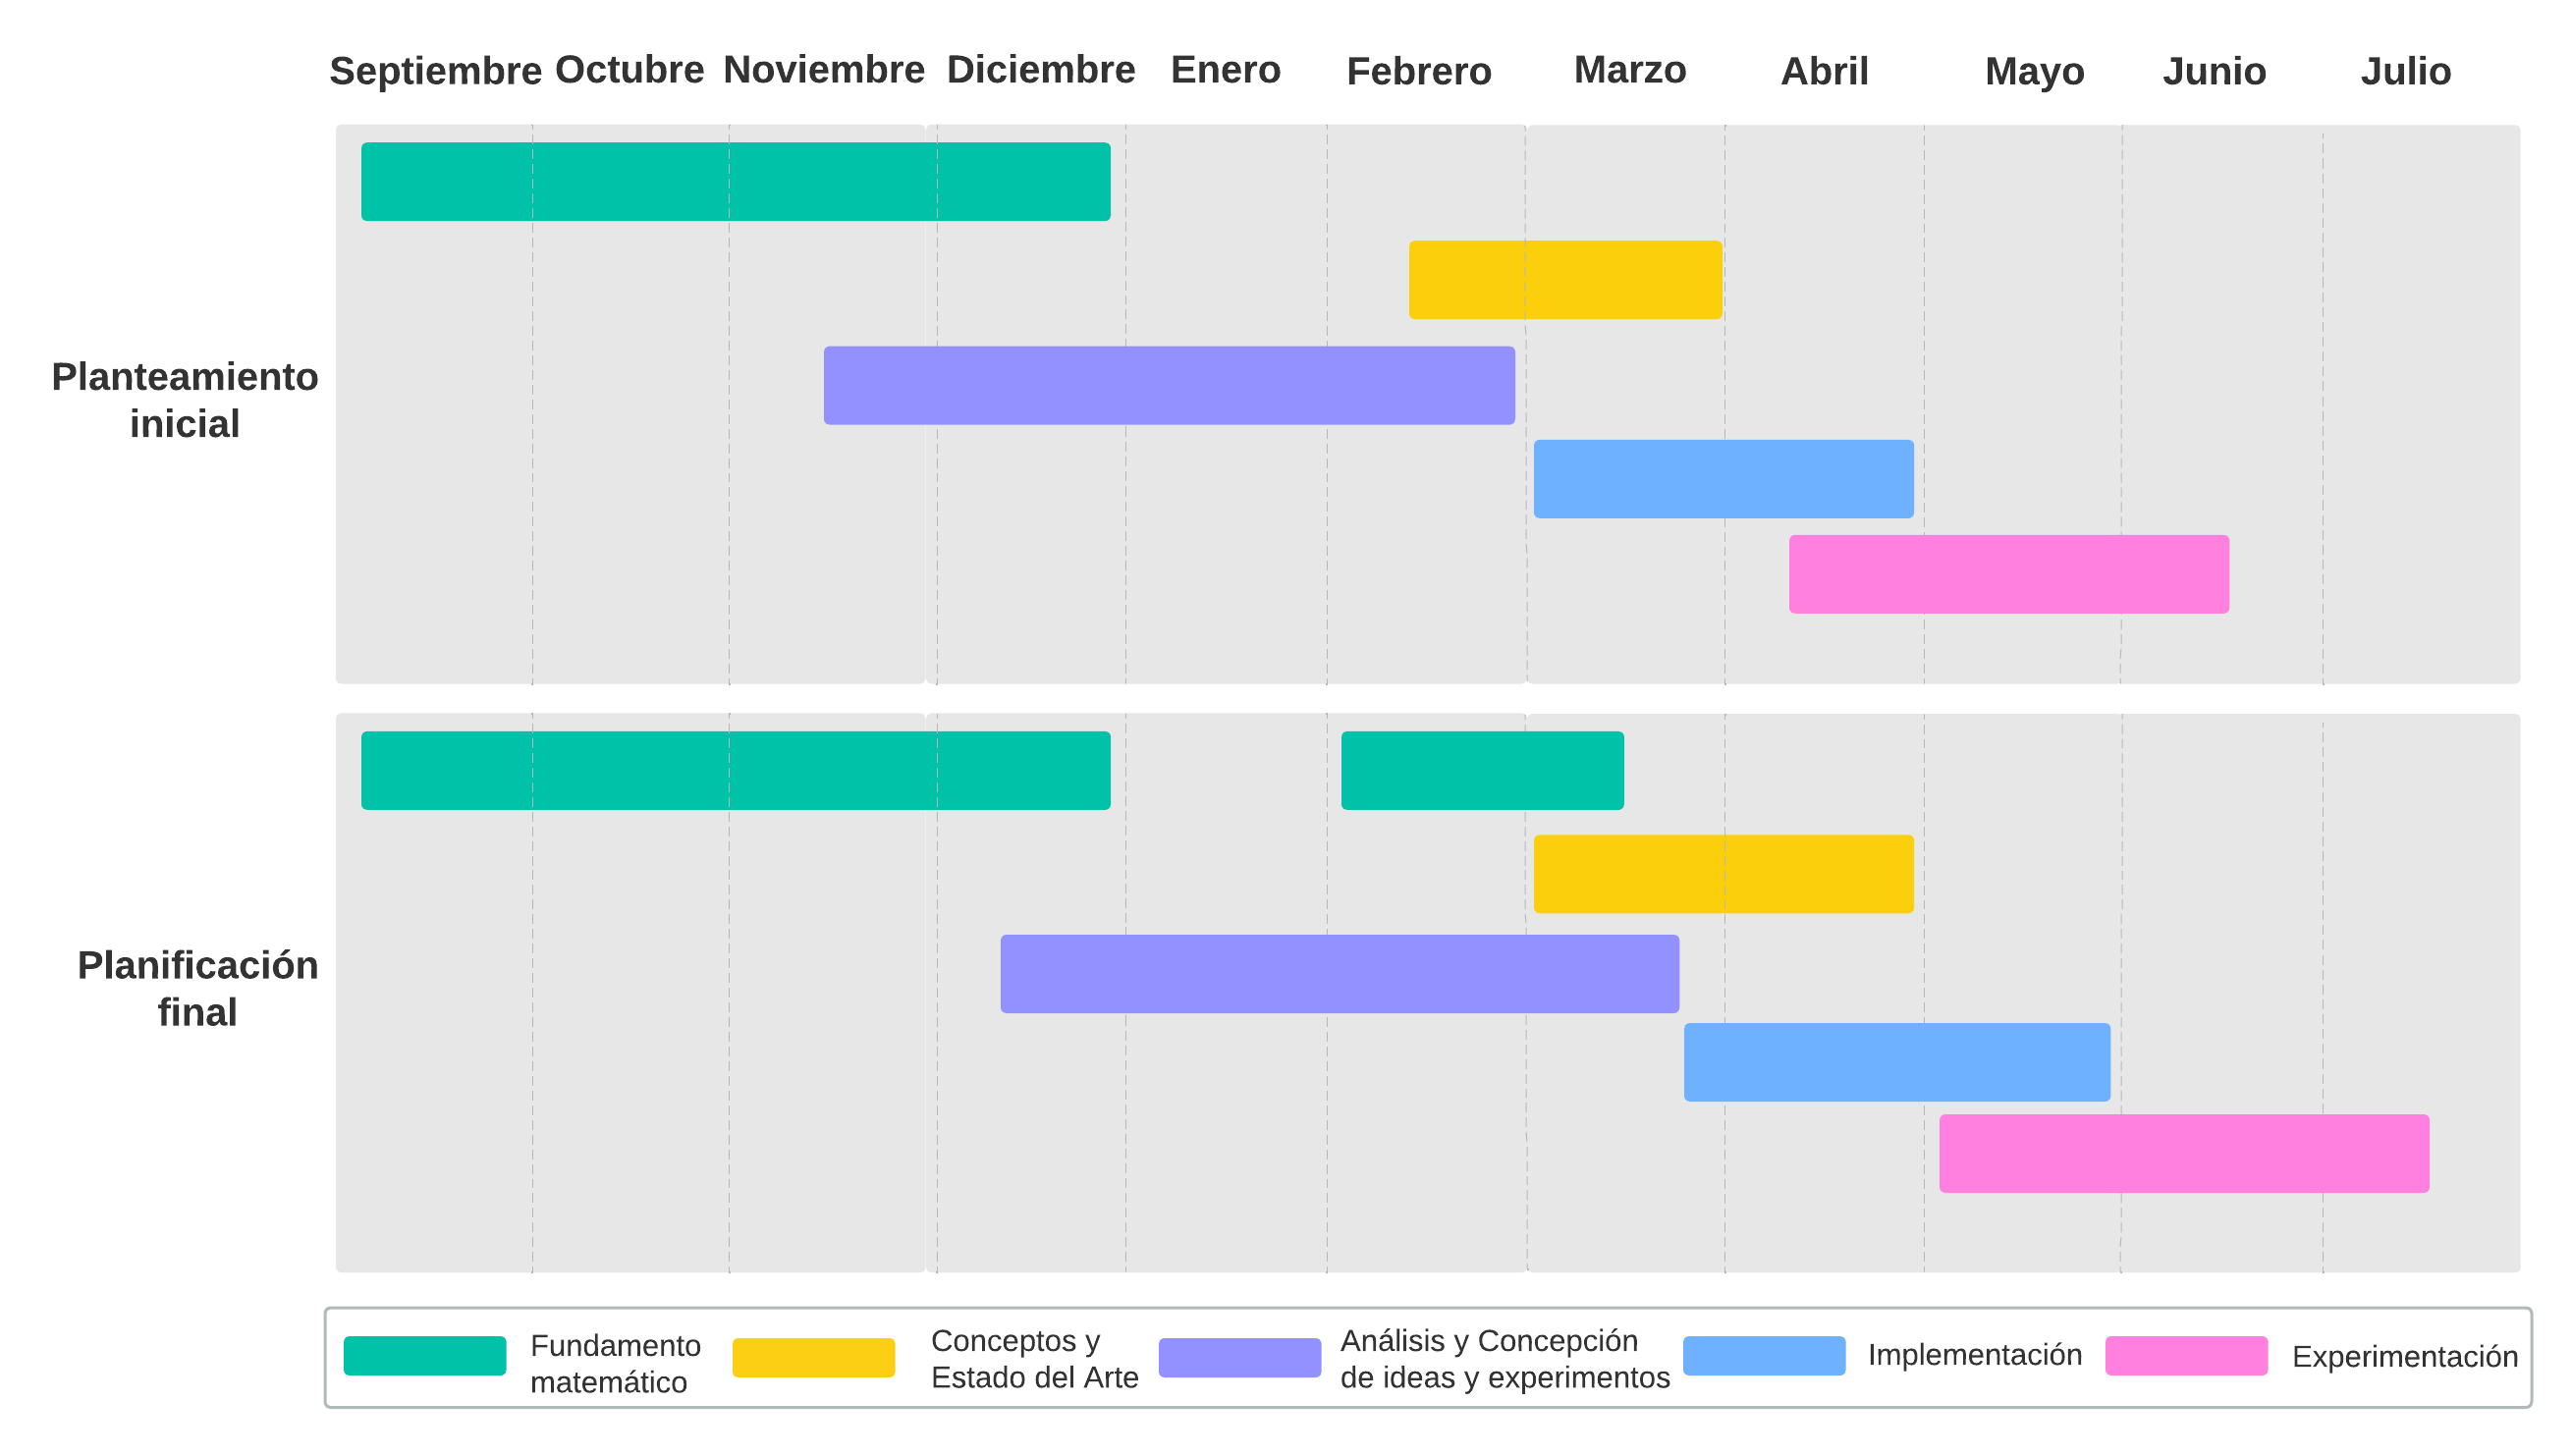
\includegraphics[width=150mm]{img/planificacion.png}
	\caption{Planificación temporal prepuesta frente a la finalmente realizada.}
	\label{fig:plan}
\end{figure}

\endinput               

% -------------------------------------------------------------------
% MAINMATTER
% -------------------------------------------------------------------
\mainmatter % activa la numeración de capítulos, resetea la numeración de las páginas y usa números arábigos

\part{Fundamento teórico} % Dividir un TFG en partes OPCIONAL
% Añadir tantos capítulos como sea necesario
% !TeX root = ../tfg.tex
% !TeX encoding = utf8

\chapter{Preliminares algebraicos}

\section{Módulos}

\begin{definicion}
	Sea $R$ un anillo cuyo elemento identidad $1 \neq 0$. Un \textbf{$R$-módulo izquierdo} $A$ es un grupo abeliano aditivo junto con una función $p: R \times A \rightarrow A$ con $(r, a) \to ra$ tal que dados $r,r' \in R$, $a,a' \in A$ se tiene
	\begin{enumerate}
		\item $(r+r')+a = ra + r'a$
		\item $(rr')a = r(r'a)$
		\item $r(a+a') = ra + ra'$
		\item $1a = a$
	\end{enumerate}
\end{definicion}

De la definición anterior se sigue que $0a = 0$ y $(-1)a = -a$.

De manera análoga, definimos \textbf{$R$-módulo derecho} donde el anillo actúa por la izquierda en vez de por la derecha de forma que $p: A \times R \rightarrow A$. Si $R$ es un anillo conmutativo, los $R$-módulos izquierdos y derechos coinciden y les llamamos simplemente $R$-módulos. Como los resultados de $R$-módulos izquierdos y derechos son análogos, trabajaremos simplemente con los $R$-módulos izquierdos y nos referiremos a ellos como $R$-módulos a menos que se indique explícitamente lo contrario.

\begin{ejemplo}
	ej
\end{ejemplo}

\begin{definicion}
	Sea $A$ un $R$-módulo izquierdo y $S$ un subconjunto de $A$. Diremos que $S$ es un submódulo izquierdo de $A$, esto es, $S \subset A$, si $S$ es cerrado respecto a la suma y si $r,s \in S$ entonces $rs \in S$. Por tanto, $S$ es un $R$-módulo.
\end{definicion}

Si un submódulo de $R$ es un subconjunto $L \subset R$ cerrado respecto a la suma tal que $rL \subset L$ para todo $r \in R$, lo llamaremos \textbf{ideal izquierdo} de $R$. Tomando un ideal izquierdo $L$ de $R$ y $A$ un $R$-módulo izquierdo, definimos el producto del ideal $L$ por el módulo $A$
\[ LA = \{\text{todas las sumas finitas } \sum l_ia_i, \text{ para } l_i \in L,\ a_i \in A \} \]
donde $LA$ es un submódulo de $A$. En particular, el producto de dos ideales izquierdos $LL'$ es también un ideal izquierdo y $(LL')A = L(L'A)$.

\begin{definicion}
	Sean $A$, $B$ $R$-módulos. Definimos el \textbf{homomorfismo de $R$-módulos} de $A$ a $B$ como la aplicación $\alpha: A \rightarrow B$ tal que
	\begin{enumerate}
		\item $\alpha(a+a') = \alpha a + \alpha a'$
		\item $\alpha(ra) = r(\alpha a)$
	\end{enumerate}
	para todo $a,a' \in A$, $r \in R$.
\end{definicion}

También es frecuente escribir el homomorfismo de $R$-módulos $\alpha: A \rightarrow B$ como $A \xrightarrow{\alpha} B$.

Cuando $\alpha: A \rightarrow B$ sea un homomorfismo de $R$-módulos, diremos que $A$ es el \textbf{dominio} y $B$ el \textbf{rango}. La \textbf{imagen} de $\alpha$ es el conjunto $\im(\alpha) = \{ \alpha(a) : a \in A \}$. El \textbf{núcleo} será el conjunto de elementos que se anulan en su imagen, esto es, $\ker(\alpha) = \{ a \in A : \alpha(a) = 0 \}$. Diremos que $\alpha$ es un \textbf{epimorfismo} cuando $\alpha(A) = B$, un \textbf{monomorfismo} cuando $\ker(\alpha) = \{0\}$ y un \textbf{isomorfismo} si $\alpha$ es un epimorfismo y un monomorfismo a la vez. Si existe un isomorfismo entre $A$ y $B$ diremos que son \textbf{isomorfos} y lo notaremos $A \cong B$. Un homomorfismo $\omega: A \rightarrow A$ lo llamaremos \textbf{endomorfismo}.

Dados dos homomorfismos de $R$-módulos $\alpha_1, \alpha_2 : A \rightarrow B$, su \textbf{suma} $\alpha_1 + \alpha_2$ la definimos como $(\alpha_1 + \alpha_2)(a) = \alpha_1(a) + \alpha_2(a)$ para todo $a \in A$. Además, dados dos homomorfismos de $R$-módulos $\alpha: A \rightarrow B$, $\beta: B \rightarrow C$, su \textbf{composición} $\beta \circ \alpha: A \rightarrow C$ es también un homomorfismo de $R$-módulos. Nótese que para que la composición sea posible, el rango de $\alpha$ tiene que ser igual al dominio de $\beta$. En ocasiones usaremos la notación $\alpha\beta = \alpha \circ \beta$. Llamaremos \textbf{inversa} (por ambos lados) de $\alpha : A \rightarrow B$ al homomorfismo $\alpha^{-1} : B \rightarrow A$ tal que $\alpha^{-1} \circ \alpha = 1_A$ y $\alpha \circ \alpha^{-1} = 1_B$. Una \textbf{inversa izquierda} de $\alpha$ es una función $\gamma: A \rightarrow A$ tal que $\gamma \circ \alpha = 1_A$. No tiene por qué existir ni ser única.

\begin{definicion}
	Sea $\{A_i, \alpha_i\}$ una familia de $R$-módulos $A_i$ y homomorfismos entre ellos tal que $\alpha_i: A_i \rightarrow A_{i+1}$. Diremos que la secuencia
	\[ \cdots \xrightarrow{\alpha_{i-2}} A_{i-1} \xrightarrow{\alpha_{i-1}} A_i \xrightarrow{\alpha_{i}} A_{i+1} \xrightarrow{\alpha_{i+1}} \cdots \]
	es \textbf{exacta} cuando $\im \alpha_i = \ker \alpha_{i+1}$.
\end{definicion}

Para cada submódulo $T \subset B$, la inclusión de $T$ en $B$ es un monomorfismo $i: T \rightarrow B$. Las \textbf{clases laterales} de $T$ en $B$ son los conjuntos $b + T = \{b + t : t \in T\}$ donde $b \in B$. Dos clases laterales $b_1 + T$, $b_2 + T$ son iguales si $b_1 - b_2 \in T$. Como $T$ es un submódulo, el grupo abeliano $B/T$ se convierte en un $R$-módulo cuando $r(b+T) = rb + T$ para todo $r \in R$. A este $R$-módulo lo llamaremos el \textbf{módulo cociente} de $B$ sobre $T$. El homomorfismo $\pi: B \rightarrow B/T$ tal que $\pi(b) = b + T$ es un epimorfismo que llamaremos \textbf{proyección canónica} de $B$.

\begin{proposicion}\label{prop:first_iso}

Sea \( \beta: B \rightarrow B' \) un homomorfismo de módulos con \( T \subset \ker \beta \). Existe entonces un único homomorfismo de módulos \( \beta': B/T \rightarrow B' \) con \( \beta'\pi = \beta \); es decir, el siguiente diagrama con \( \beta(T) = 0 \)
\[
\begin{array}{ccc}
	B & \stackrel{\pi}{\longrightarrow} & B/T \\
	& \searrow \beta & \downarrow \beta' \\
	& & B'
\end{array}
\]
es conmutativo.
\end{proposicion}

\begin{proof}
Definamos \( \beta'(b + T) = \beta(b) \). Por estar $T$ contenida en el núcleo de $\beta$, la función está bien definida. En efecto, si $a,b \in B$ entonces $a+T = b+T \Rightarrow a-b \in T \subset \ker \beta \Rightarrow \beta(a-b) = 0 \Rightarrow \beta(a)=\beta(b)$. Como $\beta$ es un homomorfismo, $\beta'$ también lo es.
\end{proof}

En particular, si \( \beta: B \rightarrow B' \) es un epimorfismo con núcleo \( T \), \( \beta': B/T \rightarrow B' \) es un isomorfismo. Esta afirmación puede expresarse de la siguiente manera: cada \( \beta \) con \( \beta(T) = 0 \) \textit{factoriza de manera única} a través de la proyección \( \pi \). Esta propiedad caracteriza a \( \pi: B \rightarrow B/T \) hasta un isomorfismo de \( B/T \), de la siguiente manera:

\begin{proposicion}
	Si \( T \subset B \) y \( \eta: B \rightarrow D \) es tal que \( \eta(T) = 0 \) y cada \( \beta: B \rightarrow B' \) con \( \beta(T) = 0 \) factoriza de manera única a través de \( \eta \), entonces hay un isomorfismo \( \theta: B/T \cong D \) con \( \theta \pi = \eta \).
\end{proposicion}

\begin{proof}
	Factorizar \(\eta\) a través de \(\pi\) y \(\pi\) a través de \(\eta\), así que \(\eta = (\eta' \pi) \eta = 1_\eta\). Pero \(\eta\) factoriza \textit{únicamente} a través de \(\pi\), así que \(\eta' \pi = 1\). Simétricamente, \(\pi' \eta = 1\). Por lo tanto \(\pi' = (\eta')^{-1}\) y \(\eta'\) es el isomorfismo deseado \(\theta\).
\end{proof}

Para cualquier \(T \subseteq B\) la inyección \(i\) y la proyección \(\pi\) producen una secuencia exacta.
\[ 0 \rightarrow T \xrightarrow{i} B \xrightarrow{\pi} B/T \rightarrow 0. \]

\begin{definicion}
Sean $A,B$ y $C$ $R$-módulos y $\sigma: A \rightarrow B$, $\gamma: B \rightarrow C$ homomorfismos entre ellos. Diremos que la secuencia 
\[ (\sigma, \gamma): 0 \rightarrow A \xrightarrow{\sigma} B \xrightarrow{\gamma} C \rightarrow 0 \]
es una \textbf{secuencia exacta corta}. Es decir, una secuencia exacta de cinco \(R\)-módulos con los dos módulos exteriores siendo cero (y por lo tanto las dos funciones exteriores triviales).
\end{definicion}

La exactitud en \(A\) significa que \(\sigma\) es un monomorfismo, en \(B\) significa que \(\sigma A = \ker \gamma\) y en \(C\) que \(\gamma\) es un epimorfismo. Así la secuencia exacta corta puede escribirse como \(A \xrightarrow{\sigma} B \xrightarrow{\gamma} C\), con exactitud en \(B\). Ahora \(\sigma\) induce un isomorfismo \(\sigma': A \to A\) y \(\gamma\) un isomorfismo \(\gamma': B/\sigma A \to C\); juntos estos proveen un isomorfismo de secuencias exactas cortas, en la forma de un diagrama conmutativo
\[
\begin{tikzcd}
	0 \arrow[r] & A \arrow[r, "\sigma"] \arrow[d, "\sigma'"] & B \arrow[r, "\gamma"] \arrow[d, no head, Rightarrow] & C \arrow[r] \arrow[d, "(\gamma')^{-1}"] & 0 \\
	0 \arrow[r] & \sigma A \arrow[r, "i"]                    & B \arrow[r]                                          & B/\sigma A \arrow[r]                    & 0
\end{tikzcd}
\]

En resumen, una secuencia exacta corta es simplemente otro nombre para un submódulo y su cociente.

%Cada homomorfismo \(\alpha: A \rightarrow B\) determina dos módulos cociente
%\[\text{Coim } \alpha = A / \text{Ker } \alpha, \quad \text{Coker } \alpha = B / \text{Im } \alpha,\]
%llamados la \textbf{coimagen} y el \textbf{conúcleo} de \(\alpha\). Esta definición provee dos secuencias exactas cortas
%\[ \text{Ker } \alpha \hookrightarrow A \twoheadrightarrow \text{Coim } \alpha, \quad \text{Im } \alpha \hookrightarrow B \twoheadrightarrow \text{Coker } \alpha, \]
%un isomorfismo \(\text{Coim } \alpha \cong \text{Im } \alpha\) y una secuencia exacta más larga
%\[ 0 \rightarrow \text{Ker } \alpha \xrightarrow{i} A \xrightarrow{\alpha} B \rightarrow \text{Coker } \alpha \rightarrow 0. \]
%
%Por la \ref{prop:first_iso}, \(\beta \alpha = 0\) implica que \(\beta\) factoriza de manera única a través de \(\pi\) como \(\beta = \beta' \pi\). Dualmente, si algún \(\gamma': A' \rightarrow A\) tiene \(\alpha \gamma' = 0\), entonces \(\gamma'\) factoriza a través de \(i\) como \(\gamma' = i \gamma''\) para un único \(\gamma'': A' \rightarrow \ker \alpha\). Esta propiedad caracteriza \(i: \ker \alpha \rightarrow A\) como un isomorfismo de \(\text{Ker } \alpha\). Observa las afirmaciones duales: \(\alpha\) es un monomorfismo si y solo si \(\ker \alpha = 0\), y es un epimorfismo si y solo si \(\text{Coker } \alpha = 0\).

Si \(\alpha: A \rightarrow B\) y \(S \subseteq A\), el conjunto \(\alpha S\) de todos los elementos \(\alpha s\) para \(s \in S\) es un submódulo de \(B\) llamado la \textbf{imagen} de \(S\) bajo \(\alpha\). De manera similar, si \(T \subseteq B\), el conjunto \(\alpha^{-1}T\) de todos los \(s \in A\) con \(\alpha s \in T\) es un submódulo de \(A\), llamada la \textbf{imagen inversa} (completa) de \(T\). En particular, \(\ker \alpha = \alpha^{-1}0\), donde \(0\) denota el submódulo de \(B\) que consiste solo del elemento cero.

Para \(K \subseteq S \subseteq A\) el módulo \(S/K\) es llamado un \textbf{subcociente} de \(A\); es un módulo cociente del submódulo \(S\) de \(A\), y simultáneamente un submódulo del módulo cociente \(A/K\). Además, si \(K' \subseteq K \subseteq S' \subseteq S \subseteq A\), entonces \(K'/K\) es un submódulo de \(S'/K\) y la proyección compuesta \(S' \rightarrow (S'/K)/(K'/K)\) tiene núcleo \(K'\), por lo tanto el isomorfismo familiar \((S'/K)/(K'/K) \cong S'/K'\). Esto nos permite escribir cada subcociente \((S'/K)/(K'/K)\) de un subcociente \(S/K\) directamente como un subcociente de \(A\). Si \( \alpha: A \rightarrow A'\) tiene \(\alpha S \subseteq S'\) y \(\alpha K \subseteq K'\), entonces \(\alpha s + K'\) es una clase lateral de \(S'/K'\) determinada de manera única por la clase lateral \(s+K\) de \(S/K\). Por lo tanto \(\alpha_{\ast}(s+K) = \alpha s + K'\) define un homomorfismo
\[\alpha_{\ast}: S/K \rightarrow S'/K'\]
\[(\alpha S \subseteq S', \alpha K \subseteq K')\]
llamado el homomorfismo \textbf{inducido} por \(\alpha\) en los subcocientes dados.

Si \(S\) y \(T\) son submódulos de \(A\), su \textbf{intersección} \(S \cap T\) (como conjuntos) es también un submódulo, así como su \textbf{unión} \(S + T\), consistiendo de todas las sumas \(s + t\) para \(s \in S\), \(t \in T\). El \textbf{teorema del isomorfismo de Noether} afirma que \(1_{A}\) induce un isomorfismo

\[ 1_{\ast}: S/(S \cap T) \cong (S + T)/T. \]

\section{Categorías}

\begin{definicion}
	Una \textbf{categoría} $\mathcal{C}$ es una tripleta $(\mathcal{O}, \hom, \circ)$ formada por
	\begin{enumerate}
		\item Una clase $\mathcal{O}$, cuyos elementos denominamos \textbf{objetos} de $\mathcal{C}$ y notamos por $Obj(\mathcal{C})$.
		\item Por cada par de objetos $(A,B)$ de $\mathcal{C}$, un conjunto $\hom(A,B)$ cuyos elementos son llamados \textbf{morfismos} de $A$ a $B$. Si $f \in \hom(A,B)$, normalmente escribiremos $f: A \rightarrow B$ o $A \xrightarrow{f} B$.
		\item Una \textbf{ley de composición} que asocia a cada morfismo $f: A \rightarrow B$ y a cada morfismo $g: B \rightarrow C$ un morfismo $g \circ f : A \rightarrow C$ satisfaciendo
		\begin{itemize}
			\item \textbf{Asociatividad}. Si $f: A \rightarrow B$, $g: B \rightarrow C$ y $h : C \rightarrow D$ son morfismos de $\mathcal{C}$, entonces $h \circ (g \circ f) = (h \circ g) \circ f$.
			\item \textbf{Identidad}. A cada objeto $B$ le podemos asociar un morfismo identidad $1_B : B \rightarrow B$ tal que si $f: A \rightarrow B$ y $g: B \rightarrow C$ entonces $g \circ 1_B = g$ y $1_B \circ f = f$.
		\end{itemize}
		Llamaremos a este morfismo la \textbf{composición} de $f$ y $g$.
	\end{enumerate}
\end{definicion}

\begin{ejemplo}
	Como veremos a continuación, la definición anterior nos va a permitir trabajar con un gran número de espacios matemáticos que ya conocemos en el contexto de la teoría de categorías. Algunos de ellos son:
	\begin{itemize}
		\item \textbf{La categoría de espacios topológicos}, donde los objetos son todos los espacios topológicos y los morfismos todas las aplicaciones continuas entre espacios topológicos $f: X \rightarrow Y$.
		\item \textbf{La categoría de grupos}, donde los objetos son todos los grupos y los morfismos todos los homomorfismos de grupos.
		\item \textbf{La categoría de conjuntos}, cuyos objetos son todos los conjuntos y sus morfismos todas las aplicaciones entre conjuntos.
	\end{itemize}
\end{ejemplo}

\begin{definicion}
	Sea $f \in \hom(A,B)$ un morfismo en la categoría $\mathcal{C}$. Diremos que $f$ es una \textbf{equivalencia} en $\mathcal{C}$ si existe en $\mathcal{C}$ otro morfismo $g \in \hom(B,A)$ tal que $g \circ f = 1_A$ y $f \circ g = 1_B$.
\end{definicion}

Nótese que si $f \in \hom(A,B)$ es una equivalencia en $\mathcal{C}$, $g \in \hom(B,A)$ debe ser única. En efecto, si suponemos que existe $g' \in \hom(B,A)$ tal que $g' \circ f = 1_A$, entonces $g = g'\circ f \circ g = g' \circ 1_B = g'$.

\section{Funtores}

\begin{definicion}
	Sean $\mathcal{C}, \mathcal{D}$ dos categorías. Un \textbf{funtor covariante} de $\mathcal{C}$ a $\mathcal{D}$ es una pareja de funciones \textit{denotadas por la misma letra $T$} tal que:
	\begin{enumerate}
		\item Una \textbf{función objeto} que asigna a cada objeto $C \in \mathcal{C}$ un objeto $T(C) \in \mathcal{D}$.
		\item Una \textbf{función de morfismos} qu asigna a cada morfismo $\gamma: C \rightarrow C'$ de $\mathcal{C}$ un morfismo $T(\gamma): T(C) \rightarrow T(C')$ de $\mathcal{D}$. Este par de funciones satisfacen las siguientes condiciones:
		\begin{equation}
			T(1_C) = 1_{T(C)}, \qquad C \in \mathcal{C},
		\end{equation}
		\begin{equation}
			T(\beta \gamma) = T(\beta)T(\gamma), \qquad \beta \gamma \text{ definido en } \mathcal{C}.
		\end{equation}
	\end{enumerate}
\end{definicion}

Es decir, un funtor covariante $T: \mathcal{C} \rightarrow \mathcal{D}$ es una aplicación que preserva el rango, dominio, identidades y composiciones de $\mathcal{C}$ en $\mathcal{D}$.

\endinput
%--------------------------------------------------------------------
% FIN DEL CAPÍTULO. 
%--------------------------------------------------------------------

% !TeX root = ../tfg.tex
% !TeX encoding = utf8

\chapter{Símplices y complejos simpliciales}

\section{Símplices}

Con la finalidad de generalizar estructuras como el triángulo y el tetraedro, 
a finales del siglo XIX nace un nuevo concepto: el símplice. Su simplicidad y 
propiedades lo convirtieron en una herramienta muy versátil en el estudio de la
topología algebraica, dando lugar a lo que hoy conocemos como homología simplicial. 
En esta sección definiremos lo que es un símplice y algunos conceptos asociados a él
que nos serán de gran utilidad en el estudio de dicho campo.

\begin{definicion}
	Sea $\{a_0, \dots, a_n\}$ un conjunto de puntos en $\mathbb{R}^N$. 
	Diremos que dicho conjunto es \textbf{afínmente independiente} si 
	para cualesquiera $t_i \in \mathbb{R}$, las ecuaciones
	\[ \sum_{i=0}^{n}t_i=0 \quad \text{y} \quad \sum_{i=0}^{n}t_ia_i=0 \]
	implican que $t_0 = t_1 = \dots = t_n$.
\end{definicion}

\begin{definicion}
	Sea $\{a_0, \dots, a_n\}$ un conjunto de puntos afínmente independiente en 
	$\mathbb{R}^N$. Definimos el \textbf{símplice} $\sigma = [a_0, \dots, a_n]$ 
	generado por $a_0, 	\dots, a_n$ como el conjunto de todos los $x \in \mathbb{R}^N$ 
	tales que
	\[ x=\sum_{i=0}^{n}t_ia_i \quad \text{y} \quad \sum_{i=0}^{n}t_i=1 \]
	con $t_i \geq 0$, $i \in \{1, \dots, n\}$.
\end{definicion}
Los coeficientes $t_i$ están determinados de manera única por el punto $x$. A los términos  
$t_0, \dots, t_n$ los llamamos las \textbf{coordenadas baricéntricas} de $\sigma$
con respecto a $a_0, \dots, a_n$.

Los puntos $a_0, \dots, a_n$ que generan $\sigma$ los llamaremos \textbf{vértices} de $\sigma$
y al número $n$ lo llamaremos la \textbf{dimensión} de $\sigma$.

\begin{definicion}
	Sea $\sigma=[a_0, \dots, a_n]$ un símplice. Una \textbf{cara} de $\sigma$ será cualquier
	símplice generado por un subconjunto de $\{a_0, \dots, a_n\}$.
\end{definicion}
En particular, la cara de $\sigma$ generada por $a_0, \dots, a_{i-1}, a_{i+1}, \dots, a_n$ la 
llamamos la \textbf{cara opuesta} de $a_i$, $i \in \{0, \dots, n\}$. Las caras de $\sigma$ 
diferentes de $\sigma$ diremos que son \textbf{caras propias} de $\sigma$ y la unión de todas ellas la 
llamaremos el \textbf{borde} de $\sigma$. Finalmente, definimos el \textbf{interior} de $\sigma$
como el conjunto de puntos de $\sigma$ que no pertenecen a su borde.

\begin{ejemplo}
\begin{figure}[h]
	\begin{minipage}{.24\textwidth}
		\centering
		{
			\begin{tikzpicture}
				% 0-símplex
				\draw (0,0);
			\end{tikzpicture}
		}\subcaption{0-símplex}
	\end{minipage}
	\begin{minipage}{.24\textwidth}
		\centering
		{
			\begin{tikzpicture}
				% 1-símplex
				\draw (0,0) -- (1,0);
			\end{tikzpicture}
		}\subcaption{1-símplex}
	\end{minipage}
	\begin{minipage}{.24\textwidth}
		\centering
		{
			\begin{tikzpicture}
				% 2-símplex
				\draw (0,0) -- (1,0) -- (0.5,0.87) -- cycle;
			\end{tikzpicture}
		}\subcaption{2-símplex}
	\end{minipage}
	\begin{minipage}{.24\textwidth}
		\centering
		{
			\begin{tikzpicture}
				% 3-símplex
				\draw (0,0) -- (1,0) -- (0.5,0.87) -- cycle;
				\draw (0.5,0.4) -- (0.5,0.87);
				\draw (0.5,0.4) -- (0,0);
				\draw (0.5,0.4) -- (1,0);
			\end{tikzpicture}
		}\subcaption{3-símplex}
	\end{minipage}
	\caption{Símplices en columnas}
\end{figure}
\end{ejemplo}

\section{Complejos simpliciales}

\begin{definicion}
	Un \textbf{complejo simplicial} $K$ en $\mathbb{R}^N$ es una colección de símplices en $\mathbb{R}^N$
	 tal que:
	\begin{enumerate}
		\item Toda cara de un símplice de $K$ está en $K$.
		\item La intersección de cualesquiera dos símplices de $K$ es una cara 
		de ambos símplices.
	\end{enumerate}
\end{definicion}

En ciertas ocasiones puede ser interesante saber si dada una colección cualquiera de símplices, esta es 
un complejo simplicial o no. Para ello, el siguiente lema nos puede ser de utilidad.

\begin{lema}
	Una colección $K$ de símplices es un complejo simplicial si, y sólo si, se cumplen las siguientes 
	condiciones:
	\begin{enumerate}
		\item Toda cara de un símplice de $K$ está en $K$.
		\item Los símplices de $K$ tienen interior disjunto dos a dos.
	\end{enumerate}
\end{lema}
\begin{proof}
	Primero, asumamos que $K$ es un complejo simplicial. MUNKRES
\end{proof}

\begin{definicion}
	Si $L$ es una subcolección del complejo simplicial $K$ que contiene todas las caras de sus 
	elementos, entonces $L$ es un complejo simplicial que llamaremos \textbf{subcomplejo} de $K$.
\end{definicion}
Entre los subcomplejos de un complejo simplicial, cabe destacar el siguiente. Diremos \textbf{p-esqueleto} 
de $K$ al subcomplejo formado por todas las caras de $K$ cuya dimensión sea menor o igual que $p$. Lo denotaremos por $K^{(p)}$. En particular, $K^{(0)}$ es el conjunto de vértices de $K$.

\begin{definicion}
	Sea $K$ un complejo simplicial de $\mathbb{R}^N$. Definimos el \textbf{politopo} de $K$ como el 
	subconjunto $|K| \subset \mathbb{R}^N$ tal que $|K|$ es la unión de todos los símplices de $K$.
\end{definicion}
Dotando a cada símplice de la topología inducida por la topología usual de $\mathbb{R}^N$, vamos a dotar ahora a $|K|$ de una topología. Diremos que un subconjunto $A \subset |K|$ es cerrado en $|K|$ si, y sólo si, $A \cap \sigma$ es cerrado en $\sigma$ para todo $\sigma \in K$. Si llamamos $T$ a la topología 
definida de esta forma, podemos ver fácilmente que $(|K|, T)$ es un espacio topológico. Claramente, $\emptyset, |K| \in T$. SEGUIR DEMOSTRANDO

Llamaremos \textbf{poliedro} a cualquier espacio topológico que sea el politopo de un complejo simplicial.

\begin{definicion}
	Un espacio topológico $X$ es \textbf{triangulable} si existe un complejo simplicial $K$ cuyo espacio subyacente (DEFINIR ESPACIO SUBYACENTE) es homeomorfo a $X$. Diremos entonces que $h: |K| \rightarrow X$ es una \textbf{triangulación}. BUSCAR BIBLIOGRAFIA PARA ESTO
\end{definicion}

TAL VEZ ALGUNAS PROPIEDADES LOCALMENTE COMPACTO Y EJEMPLO

\section{Aplicaciones simpliciales}

Cuando trabajemos con complejos simpliciales, será interesante tener en cuenta cuándo las 
transformaciones entre ellos pueden ser continuas o incluso homeomorfismos. 

\begin{lema}
	Sean $K$ y $L$ dos complejos simpliciales y sea $f: K^{(0)} \rightarrow L^{(0)}$ una aplicación. 
	Supongamos que siempre que los vértices $v_0, \dots, v_n$ de $K$ generen un símplice en $K$, 
	los puntos $f(v_0), \dots, f(v_n)$ son vértices de un símplice de $L$. Entonces podemos extender $f$ 
	a una aplicación continua $g:|K| \rightarrow |L|$ tal que
	\[ x = \sum_{i=0}^{n}t_iv_i \quad \implies \quad g(x) = \sum_{i=0}^{n}t_if(v_i) \]
\end{lema}
Llamaremos a $g$ la \textbf{aplicación simplicial} (lineal) inducida por $f$.
\begin{proof}
	Por hipótesis, los vértices $f(v_0), \dots, f(v_n)$ generan un símplice $\tau$ en $L$. Por 
	ser $K$ un complejo simplicial, la suma de sus coeficientes $t_i$, con $i \in \{0, \dots, n\}$,  
	es igual a uno, luego $g(x) = \sum_{i=0}^{n}t_if(v_i)$ es un punto de $\tau$. Podemos ver que 
	$g$ es una aplicación continua del símplice $\sigma$ generado por $v_0, \dots, v_n$ al símplice 
	$\tau$ generado por $f(v_0), \dots, f(v_n)$.
	
	Ahora tan solo nos queda ver que $g:|K| \rightarrow |L|$ es continua. Bien, pues por ser 
	$g: \sigma \rightarrow \tau$ continua, también lo es $g: \sigma \rightarrow |L|$. Finalmente 
	por el lema METER LEMA ANTERIOR 2.3 DE MUNKRES, $g:|K| \rightarrow |L|$ es continua.
\end{proof}

\begin{lema}\label{lem:homeo_complex}
	Supongamos que $f:K^{(0)} \rightarrow L^{(0)}$ es una aplicación biyectiva tal que los vértices 
	$v_0, \dots, v_n$ de $K$ generan un símplice de $K$ si, y sólo si, $f(v_0), \dots, f(v_n)$ 
	generan un símplice de $L$. Entonces la aplicación simplicial inducida $g:|K| \rightarrow |L|$ 
	es un homeomorfismo.
\end{lema}
Diremos entonces que $g$ es un \textbf{homeomorfismo simplicial} de $K$ con $L$.
\begin{proof}
	Por hipótesis, cada símplice $\sigma \in K$ se identifica con otro símplice $\tau \in L$. 
	Por tanto, debemos comprobar que la aplicación lineal $h: \tau \rightarrow \sigma$ inducida por 
	la correspondencia de vértices $f^{-1}$ es la inversa de $g: \sigma \rightarrow \tau$. Si 
	consideramos $x = \sum_{i=0}^{n}t_i v_i$, entonces por definición $g(x) = \sum_{i=0}^{n}t_if(v_i)$.
	Luego
	\[ h(g(x)) = h(\sum_{i=0}^{n}t_if(v_i)) = \sum_{i=0}^{n}t_i f^{-1}(v_i) = \sum_{i=0}^{n}t_i v_i = x \]
	
\end{proof}

\section{Complejos simpliciales abstractos}

Si bien la definición actual de los complejos simpliciales puede llegar a ser de gran utilidad, en 
la práctica muchas veces no es necesario usar las herramientas que nos proporciona la geometría afín. 
Es por ello que vamos a introducir una descripción puramente combinatoria de los complejos simpliciales 
que, aun siendo más simples, son de gran utilidad a la hora de trabajar con espacios topológicos.

\begin{definicion}
	Un \textbf{complejo simplicial abstracto} (o simplemente complejo abstracto) es una 
	colección $\mathcal{S}$ de conjuntos finitos no vacíos tal que si $A \in \mathcal{S}$, 
	entonces para todo $B \subset A$ con $B$ no vacío, $B \in \mathcal{S}$.
\end{definicion}

Al elemento $A$ de $\mathcal{S}$ lo llamaremos \textbf{símplice} de $A \in \mathcal{S}$. La 
\textbf{dimensión} de $A$ es una menos que el número de elementos que le pertenecen. Todo 
subconjunto de $A$ lo llamaremos \textbf{cara} de $A$. En cuanto a la \textbf{dimensión} de 
$\mathcal{S}$, diremos que es igual al máximo de las dimensiones de sus elementos o en caso de 
no haberlo, diremos que la dimensión de $\mathcal{S}$ es infinita. El \textbf{conjunto de vértices} 
$V$ de $\mathcal{S}$ diremos que es la unión de elementos de $\mathcal{S}$ que contienen un único punto. 
Llamaremos \textbf{subcomplejo} de $\mathcal{S}$ a cualquier subcolección de $\mathcal{S}$ que sea 
un complejo simplicial abstracto en sí.

Sean $V_S$, $V_T$ los conjuntos de vértices de los complejos abstractos $\mathcal{S}$, $\mathcal{T}$  respectivamente. Dos complejos abstractos $\mathcal{S}$ y $\mathcal{T}$ diremos que son 
\textbf{isomorfos} si existe una aplicación biyectiva $f: V_S \rightarrow V_T$ tal que 
$\{a_0, \dots, a_n\} \in \mathcal{S}$ si, y sólo si, $\{f(a_0), \dots, f(a_n)\} \in \mathcal{T}$.

\begin{definicion}
	Sean $K$ un complejo simplicial y $V$ su conjunto de vértices. Sea $\mathcal{K}$ la colección de 
	todos los subconjuntos $\{a_0, \dots, a_n\} \subset V$ tales que los vértices $a_0, \dots, a_n$ 
	generan un símplice de $K$. Entonces llamaremos a la colección $\mathcal{K}$ el 
	\textbf{esquema de vértices} de $K$.
\end{definicion}

Después de realizar todas las definiciones pertinentes, ya estamos en condiciones de enunciar el 
siguiente teorema.

\begin{teorema}
	Las siguientes afirmaciones son ciertas:
	\begin{enumerate}[label=(\alph*)]
		\item Todo complejo abstracto $\mathcal{S}$ es isomorfo al esquema de vértices de algún 
		complejo simplicial $K$.
		\item Dos complejos simpliciales son linealmente isomorfos si, y sólo si, sus esquemas 
		de vértices son isomorfos como complejos simpliciales abstractos.
	\end{enumerate}
\end{teorema}
\begin{proof}
	Para demostrar $(a)$, empezaremos tomando un conjunto de índices $J$. Llamemos $\mathbf{E}^J$ 
	al subconjunto de funciones $x: J \rightarrow \mathbb{R}$ de $\mathbb{R}^J$ tales que $x(\alpha) = 0$ 
	para todo $\alpha \in J$ excepto para un número finito de valores. Sea $\Delta^J$ la 
	colección de todos los símplices en $\mathbf{E}^J$ generados por subconjuntos finitos de 
	la base usual de $\mathbf{E}^J$. $\Delta^J$ es un complejo simplicial. 
	Sean entonces $\sigma, \tau$ símplices de $\Delta^J$, la 
	unión de sus conjuntos de vértices es afínmente independiente y genera un símplice en $\Delta^J$.
	Diremos que $\Delta^J$ es un \textit{símplice de dimensión infinita}.
	
	Sea ahora $\mathcal{S}$ un complejo abstracto con conjunto de vértices $V$. Tomamos un conjunto 
	de índices $J$ lo bastante grande para que podamos tomar una aplicación inyectiva 
	$f: V \rightarrow J$. A continuación, vamos a tomar un subcomplejo de $\Delta^J$ tal que para 
	cada símplice abstracto $\{a_0, \dots, a_n\} \in \mathcal{S}$, el símplice (geométrico) generado 
	por $f(a_0), \dots, f(a_n)$ está en $K$. Por tanto $K$ es un complejo simplicial y 
	$f$ es un isomorfismo entre $\mathcal{S}$ y el esquema de vértices de $K$.
	
	En cuanto a $(b)$, es una consecuencia inmediata del \autoref{lem:homeo_complex}
\end{proof}

\begin{definicion}
	Si el complejo simplicial abstracto $\mathcal{S}$ es isomorfo al esquema de vértices del 
	complejo simplicial $K$, diremos que $K$ es una \textbf{realización geométrica} de $\mathcal{S}$.
\end{definicion}

\begin{lema}
	Sea $\mathcal{S}$ un comlpejo simplicial abstracto de dimensión $d$. Entonces $\mathcal{S}$ tiene 
	una realización geométrica en $\mathbb{R}^{2d+1}$.
\end{lema}
\begin{proof}
	TENGO LA DEMOSTRACION EN TDA PERO HAY QUE BUSCAR OTRA FUENTE.
\end{proof}

\begin{ejemplo}
	ALGUN EJEMPLO QUE MUESTRE SU UTILIDAD.
\end{ejemplo}

\section{Triangulaciones}



\section{Algunos complejos simpliciales}

\endinput
%--------------------------------------------------------------------
% FIN DEL CAPÍTULO. 
%--------------------------------------------------------------------

% !TeX root = ../tfg.tex
% !TeX encoding = utf8

\chapter{Homología}

El término de homología se puede definir de manera puramente algebraica, lo cual marcó un avance significativo en el desarrollo de la topología algebraica. En este capítulo, presentaremos una síntesis concisa de los fundamentos que subyacen a las diversas aproximaciones para construir la teoría de la homología. Estos principios servirán como base para abordar casos específicos en capítulos posteriores y comprender mejor las propiedades topológicas de los espacios.

\section{Grupos de homología}

\begin{definicion}
	Sea $C$ un grupo abeliano junto a un endomorfismo  $d: C \rightarrow C$ tal que $d^2 = 0$. Diremos entonces que $C$ es un \textbf{grupo diferencial} y llamaremos a $d$ \textbf{operador borde} de $C$.
\end{definicion}

Llamaremos a los elementos de $C$ \textbf{cadenas}. El subgrupo de \textbf{ciclos} será $Z(C) = \ker d$,  y el subgrupo de \textbf{bordes} $B(C) = \im d$. Si nos fijamos, el requisito $d^2 = 0$ es equivalente a exigir que $\im{d} \subset \ker{d}$.

\begin{definicion}
	Sea $C$ un grupo diferencial. Definimos el \textbf{grupo de homología} de $C$ como el grupo cociente $H(C)$ tal que 
	\[ H(C) = \frac{Z(C)}{B(C)}\]
\end{definicion}

Por tanto, el grupo de homología de un grupo diferencial $C$ está formado por las clases laterales $[c] = c + B(C)$ donde $c$ es un ciclo de $C$. A los elementos de $H(C)$ los llamaremos \textbf{clases de homología}. Dos ciclos $c$ y $c'$ diremos que son \textbf{homólogos} si ambos pertenecen a la misma clase de homología, esto es, $c \sim c'$.

\begin{ejemplo}
	contenidos...
\end{ejemplo}

\begin{definicion}
	Sean $C$ y $C'$ dos grupos diferenciales y $d, d'$ sus respectivos operadores borde. Diremos que $f: C \rightarrow C'$ es un \textbf{homomorfismo de grupos diferenciales} si $f$ es un homomorfismo de grupos y además $d'f = fd$.
\end{definicion}

La anterior definición nos permite preservar la estructura algebraica del grupo diferencial. De esta forma, si tomamos una cadena $c \in C$ que sea un ciclo o un borde y $f:C \rightarrow C'$ es un homomorfismo de grupos diferenciales, $f(c) \in C'$ seguirá siendo un ciclo o un borde de manera correspondiente.

\begin{definicion}
	Sean $C, C'$ grupos diferenciales y $f:C \rightarrow C'$ un homomorfismo de grupos diferenciales. Definimos la función $f_* = H(f): H(C) \rightarrow H(C')$ satisfaciendo 
	\[f_*([c]) = [f(c)] \]
	Diremos que $H(f)$ es el \textbf{homomorfismo inducido} por $f$.
\end{definicion}

En estas condiciones, $H$ es un funtor covariante de la categoría de grupos diferenciales a la categoría de grupos.

\begin{ejemplo}
	contenidos...
\end{ejemplo}

\section{Complejos de cadena}

\begin{definicion}
	Sea $R$ un anillo. Un \textbf{complejo de cadenas} $K$ de $R$-módulos es una familia $\{K_n, \partial_n\}$ donde $K_n$ son $R$-módulos y $\partial_n : K_n \rightarrow K_{n-1}$ homomorfismos de $R$-módulos tales que $\partial_n \partial_{n-1} = 0$ para todo $n \in \mathbb{Z}$.
\end{definicion}

La última condición es equivalente a que $\im{\partial_{n+1}} \subset \ker{\partial_n}$.

Un complejo $K$  es por tanto una secuencia doblemente infinita
\[ K : \cdots \rightarrow K_{1} \rightarrow K_0 \rightarrow K_{-1} \rightarrow \cdots \]
donde toda composición es el homomorfismo con imagen el cero. La \textbf{homología} $H(K)$ es la familia de módulos
\[ H_n(K) = \frac{\ker \partial_n}{\im \partial_{n+1}} \]
Luego $H_n(K)=0$ implica que la secuencia $K$ es exacta en $K_n$. A los elementos de $K_n$ los llamaremos \textbf{n-cadenas} o \textbf{cadenas de dimensión n}. Si la dimensión se sobrentiende, la llamaremos simplemente \textbf{cadena}. Un \textbf{n-ciclo} de $K$ es un elemento del submódulo $C_n(K) = \ker \partial_n$. Un \textbf{n-borde} es un elemento de $\partial_{n+1}K_{n+1}$. La clase lateral de un ciclo $c$ se escribe $[c] = c + \partial K_{n+1}$. Dos $n$-ciclos $c,c' \in C_n(K)$ pertenecientes a la misma clase lateral $[c]$ decimos que son \textbf{homólogos}, es decir, $c \sim c'$.

\begin{definicion}
	Sean $K,K'$ complejos de cadena. Una \textbf{aplicación de cadena} o \textbf{morfismo de cadena} $f: K \rightarrow K'$ es una familia de homomorfismos de $R$-módulos $f_n: K_n \rightarrow K_n'$ tal que $\partial_n'f_n = f_{n-1}\partial_n$ para todo $n \in \mathbb{Z}$.
\end{definicion}

La función $H_n(f) = f_*$ definida por $f_*([c]) = f_*(c + \partial K_{n+1}) = fc + \partial K'_{n+1}$ es un homomorfismo $H_n(f): H_n(K) \rightarrow H_n(K')$. Así mismo, cada $H_n$ es un funtor covariante de la categoría de complejos de cadena y morfismos de cadenas a la categoría de módulos.

\begin{definicion}\label{def:chain_homotopy}
	Sean $K,K'$ cadenas de complejos y $f,g: K \rightarrow K'$ dos aplicaciones de cadena entre ellos. Una \textbf{homotopía de cadenas} u \textbf{homotopía algebraica} $s$ es una familia de homomorfismos de módulos $s_n: K_n \rightarrow K_{n+1}'$ para cada dimensión $n \in \mathbb{Z}$ tal que
	\begin{equation}
		\partial_{n+1}'s_n + s_{n-1} \partial_n = f_n - g_n
	\end{equation}
	Diremos entonces que $f$ y $g$ son \textbf{algebraicamente homotópicas} y escribiremos $f \simeq g$.
\end{definicion}

\begin{teorema}
	Si $s$ es una homotopía de cadenas entre $f,g: K \rightarrow K'$, entonces
	\[ H_n(f) = H_n(g) : H_n(K) \rightarrow H_n(K') \]
\end{teorema}
\begin{proof}
	Si $c$ es un ciclo de $K_n$, tenemos que $\partial_n c = 0$. Por \ref{def:chain_homotopy} se cumple que $f_nc-g_nc =  \partial s_n c$. Como consecuencia $f_n c$ y $g_n c$ son homólogos lo que implica que $[f_nc] = [g_n c]$ en $H_n(K')$, como queríamos demostrar.
\end{proof}

\begin{definicion}
	Una aplicación de cadena $f: K \rightarrow K'$ es una \textbf{equivalencia de cadena} si existe otra aplicación $h: K' \rightarrow K$ y homotopías $s: h \circ f \rightarrow 1_K$, $t: f \circ h \rightarrow 1_{K'}$ tales que $h \circ f \simeq 1_K$, $f \circ h \simeq 1_{K'}$.
\end{definicion}

Como $H_n(1_K) = 1$, del anterior teorema se deduce lo siguiente.

\begin{corolario}
	Si $f: K \rightarrow K'$ es una equivalencia de cadenas, la aplicación inducida $H_n(f): H_n(K) \rightarrow H_n(K')$ es un isomorfismo para cada dimensión $n \in \mathbb{Z}$.
\end{corolario}

\begin{proposicion}
	Sean $f,g: K \rightarrow K'$ y $f',g': K' \rightarrow K''$ aplicaciones de cadena. Sean $s: f \rightarrow g$, $s': f' \rightarrow g'$ homotopías de cadena entre ellas tales que $f \simeq g$, $f' \simeq g'$. Entonces su composición
	\[ f' s + s' g: f' \circ f \rightarrow g' \circ g \qquad g' \circ g : K \rightarrow K'' \]
	es una homotopía de cadena.
\end{proposicion}
\begin{proof}
	Por ser $s,s'$ homotopías de cadena tenemos que $\partial s + s\partial = f-g$ y $\partial s' + s'\partial = f'-g'$. Aplicando  $f'$ a la izquierda de la primera expresión y $g$ a la derecha de la segunda nos queda
	\[ f'\partial s + f's\partial = f' \circ f-f' \circ g \]
	\[ \partial s' g + s'\partial g = f' \circ g-g' \circ g \]
	Sumando ambas igualdades
	\[ f'\partial s + f's\partial + \partial s' g + s'\partial g = f' \circ f-f' \circ g + f' \circ g-g' \circ g \]
	\[ f'\partial s + f's\partial + \partial s' g + s'\partial g = f' \circ f - g' \circ g \]
	\[ \partial f' s + f's \partial + \partial s' g + s' g \partial = f' \circ f - g' \circ g \]
	\[ \partial (f' s + s' g) + (f's + s' g) \partial = f' \circ f - g' \circ g \]
\end{proof}



\endinput
%--------------------------------------------------------------------
% FIN DEL CAPÍTULO. 
%--------------------------------------------------------------------


%\cleardoublepage\part{Segunda parte}
%% !TeX root = ../tfg.tex
% !TeX encoding = utf8

\chapter{Ejemplo de capítulo}

\section{Primera sección}

Este fichero \texttt{capitulo-ejemplo.tex} es una plantilla para añadir capítulos al \textsc{tfg}. Para ello, es necesario:
\begin{itemize}
  \item Crear una copia de este fichero \texttt{capitulo-ejemplo.tex} en la carpeta \texttt{capitulos} con un nombre apropiado (p.e. \texttt{capitulo01.tex}).
  \item Añadir el comando \texttt{$\backslash$input\{capitulos/capitulo01\}} en el fichero principal \texttt{tfg.tex} donde queremos que aparezca dicho capítulo.
\end{itemize}


\endinput
%--------------------------------------------------------------------
% FIN DEL CAPÍTULO. 
%--------------------------------------------------------------------


% -------------------------------------------------------------------
% APPENDIX: Opcional
% -------------------------------------------------------------------

\appendix % Reinicia la numeración de los capítulos y usa letras para numerarlos
\pdfbookmark[-1]{Apéndices}{appendix} % Alternativamente podemos agrupar los apéndices con un nuevo \part{Apéndices}

% !TeX root = ../tfg.tex
% !TeX encoding = utf8

\chapter{Ejemplo de apéndice}\label{ap:apendice1}

Los apéndices son opcionales.

Este fichero \texttt{apendice-ejemplo.tex} es una plantilla para añadir apéndices al \textsc{tfg}. Para ello, es necesario:
\begin{itemize}
  \item Crear una copia de este fichero \texttt{apendice-ejemplo.tex} en la carpeta \texttt{apendices} con un nombre apropiado (p.e. \texttt{apendice01.tex}).
  \item Añadir el comando \texttt{$\backslash$input\{apendices/apendice01\}} en el fichero principal \texttt{tfg.tex} donde queremos que aparezca dicho apéndice (debe de ser después del comando \texttt{$\backslash$appendix}).
\end{itemize}

\endinput
%------------------------------------------------------------------------------------
% FIN DEL APÉNDICE. 
%------------------------------------------------------------------------------------

% Añadir tantos apéndices como sea necesario 

% -------------------------------------------------------------------
% GLOSARIO: Opcional
% -------------------------------------------------------------------

% !TeX root = ../tfg.tex
% !TeX encoding = utf8

\chapter*{Glosario}
\addcontentsline{toc}{chapter}{Glosario} % Añade el glosario a la tabla de contenidos

La inclusión de un glosario es opcional.

Archivo: \texttt{glosario.tex}

\begin{description} 
  \item[$\mathbb{R}$] Conjunto de números reales.

  \item[$\mathbb{C}$] Conjunto de números complejos.

  \item[$\mathbb{Z}$] Conjunto de números enteros.
\end{description}
\endinput
 

% -------------------------------------------------------------------
% BACKMATTER
% -------------------------------------------------------------------

\backmatter % Desactiva la numeración de los capítulos
\pdfbookmark[-1]{Referencias}{BM-Referencias}

% BIBLIOGRAFÍA
%-------------------------------------------------------------------

\bibliographystyle{alpha-es} 
\begin{small} 
  \bibliography{library.bib}
\end{small}


\end{document}
